\documentclass{standalone}

\usepackage{tikz}
\begin{document}
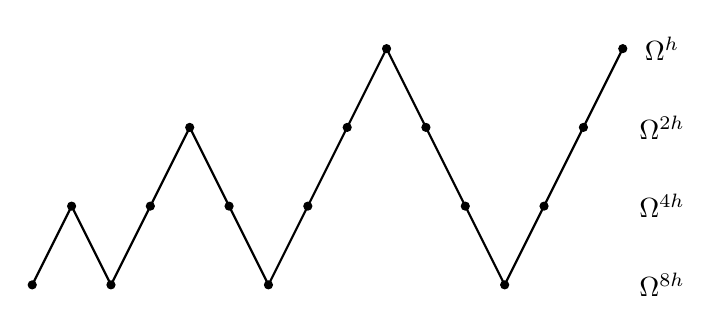
\begin{tikzpicture}
  \filldraw (0, 0) circle (0.02in);
  \filldraw (.5, 1) circle (0.02in);
  \filldraw (1, 0) circle (0.02in);
  \filldraw (1.5, 1) circle (0.02in);
  \filldraw (2, 2) circle (0.02in);
  \filldraw (2.5, 1) circle (0.02in);
  \filldraw (3, 0) circle (0.02in);
  \filldraw (3.5, 1) circle (0.02in);
  \filldraw (4.0, 2) circle (0.02in);
  \filldraw (4.5, 3) circle (0.02in);
  \filldraw (5.0, 2) circle (0.02in);
  \filldraw (5.5, 1) circle (0.02in);
  \filldraw (6, 0) circle (0.02in);
  \filldraw (6.5, 1) circle (0.02in);
  \filldraw (7.0, 2) circle (0.02in);
  \filldraw (7.5, 3) circle (0.02in);
  \draw[thick] (0, 0) -- (0.5,1);
  \draw[thick] (0.5, 1) -- (1,0);
  \draw[thick] (1, 0) -- (2,2);
  \draw[thick] (2, 2) -- (3,0);
  \draw[thick] (3, 0) -- (4.5,3);
  \draw[thick] (4.5, 3) -- (6,0);
  \draw[thick] (6, 0) -- (7.5,3);
  \node at (8, 3)  {$\Omega^h$};
  \node at (8, 2)  {$\Omega^{2h}$};
  \node at (8, 1)  {$\Omega^{4h}$};
  \node at (8, 0)  {$\Omega^{8h}$};
\end{tikzpicture}
\end{document}
  % \node at (4, 3)  {$\Omega^h$};
  % \node at (4, 2)  {$\Omega^{2h}$};
  % \node at (4, 1)  {$\Omega^{4h}$};
  % \node at (4, 0)  {$\Omega^{8h}$};
\end{tikzpicture}
\end{document}